%--------------------------------------------------------------------------------
\documentclass[12pt]{article}
%--------------------------------------------------------------------------------
\usepackage{sbc-template}
\usepackage{graphicx,url}
\usepackage[utf8]{inputenc}
\usepackage[brazil]{babel}
\usepackage{amsmath}
\usepackage[portuguese,ruled,vlined]{algorithm2e}
\usepackage{blindtext}
\usepackage{xcolor}
\usepackage{caption}
\usepackage{subcaption}
\usepackage{colortbl}
\usepackage{adjustbox}
\usepackage{tikz}
\usepackage{pgf}
\usepackage{multirow}
\usepackage{pgfplots}
\usepackage{amsmath}
\usepackage{float}
%--------------------------------------------------------------------------------
\definecolor{green}{HTML}{4CAF50}     

\sloppy

\title{Componentes Conexos em Processador \emph{Multicore}}
\author{Patreze A. Chita \inst{1}, Nahri. B. Moreano\inst{1}}
\address{Faculdade de Computação -- Universidade Federal do Mato Grosso do Sul (UFMS) %\\ Caixa Postal 549 -- 79.070.900 -- Campo Grande -- MS -- Brazil
\email{patrezechita@gmail.com, nahri@facom.ufms.br}
}

%--------------------------------------------------------------------------------
\begin{document} 

\maketitle

\begin{resumo} 
Este artigo descreve dois algoritmos encontrados na literatura, um sequencial e outro paralelo, para solucionar o problema dos componentes conexos de um grafo não orientado. Uma implementação do algoritmo paralelo é desenvolvida usando o modelo OpenMP, para execução em um processador \emph{multicore}. Os resultados são analisados através de uma avaliação experimental de desempenho.
\end{resumo}

\begin{abstract} 
This paper describes two algorithms from the literature, a sequential and a parallel one, to solve the connected components problem in an undirected graph. An implementation of the parallel algorithm is developed using the OpenMP model, for execution on a multicore processor. The results are analyzed through an experimental performance evaluation.
\end{abstract}

%--------------------------------------------------------------------------------
\section{Introdução}

Seja um grafo G=(V, E) não orientado, G é conexo se, para qualquer par \{v, u\} de vértices de V, existe um caminho com extremos v e u. Um componente conexo de um grafo G é qualquer subgrafo conexo maximal de G. Sendo assim, cada vértice de um grafo G pertence a um único componente.

Encontrar os componentes conexos de um grafo é o passo principal de muitas das aplicações com grafos. Por exemplo, considere o problema de identificar grupos em um conjunto de itens. Podemos representar cada item por um vértice e adicionar uma aresta entre par de itens que são considerados semelhantes. Os componentes conexos desse grafo correspondem a diferentes classes de itens~\cite{Skiena:2008}.

O objetivo deste trabalho é implementar e analisar duas soluções para o problema dos componentes conexos, sendo uma sequencial e outra paralela, ambas da literatura. Analisando o desempenho obtido pelos algoritmos, pretende-se concluir se a paralelização da solução de fato produz algum ganho em relação ao algoritmo sequencial.

No Capítulo~\ref{algoritmos} são descritos os dois algoritmos, sequencial e paralelo, conforme encontrados na literatura. O Capítulo~\ref{paralelo} apresenta a implementação desenvolvida do algoritmo paralelo. No Capítulo~\ref{resultados} é feita uma avaliação experimental de desempenho dos dois algoritmos e os resultados são analisados. Finalmente, o Capítulo~\ref{conclusao} apresenta a conclusão deste trabalho.

%--------------------------------------------------------------------------------
\section{Algoritmos Sequencial e Paralelo para Componentes Conexos}
\label{algoritmos}

O algoritmo sequencial para o problema dos componentes conexos utilizado neste trabalho é baseado na busca em profundidade (\emph{Depth-First Search} -- DFS). Outras técnicas podem ser utilizadas na construção de algoritmos para componentes conexos, como por exemplo, o algoritmo baseado nas operações \emph{Union-Find}. Os algoritmos baseados tanto na busca em profundidade quanto nas operações \emph{Union-Find} são descritos em~\cite{Sedgewick:2011} e~\cite{Cormen:2009}.

Em~\cite{Grama:2003} é descrito de maneira alto nível um algoritmo para componentes conexos que utiliza tanto a busca em profundidade quanto as operações \emph{Union-Find}. Outros algoritmos paralelos para esse problema podem ser encontrados em~\cite{Roosta:1999}.

%--------------------------------------------------------------------------------
\subsection{Algoritmo Sequencial Baseado em Busca em Profundidade}

Uma maneira natural de se resolver o problema dos componentes conexos de um determinado grafo é executar uma busca em profundidade no mesmo. O resultado disso é uma floresta composta por várias árvores, que são, por definição, conexas e acíclicas. Portanto, um algoritmo de busca em profundidade levemente modificado resolve o problema dos componentes conexos~\cite{Grama:2003, Sedgewick:2011}. Como resultado da busca em profundidade, todo vértice que pertence a uma mesma árvore, está em um mesmo componente do grafo. 
%Nota-se que isso é verdade, pois, partindo de um vértice, será acessado outro que compartilha uma aresta, portanto, existe um caminho entre esses dois vértices. 
A modificação necessária no algoritmo de busca em profundidade é que, toda vez que um vértice é visitado pela busca, todos os vértices alcançados a partir dele estarão no mesmo componente conexo. O Algoritmo~\ref{alg_seq} mostra essa solução sequencial, baseada na busca em profundidade, com a modificação para se obter a informação de a qual componente cada vértice pertence. A complexidade de tempo desse algoritmo é O($|\text{V}|+|\text{E}|$).

\begin{algorithm}[!htb]
    \DontPrintSemicolon
    \SetArgSty{textnormal}
    \caption{Algoritmo sequencial para componentes conexos}
    \label{alg_seq}
    \SetKwProg{ComponentesConexos}{ComponentesConexos}{}{}
    \ComponentesConexos{{\normalfont(grafo G = (V, E))}}
	{
        nComponentes $\gets$ 0\;
        \ParaCada{vértice v $\in$ V}
        {
            visitado[v] $\gets$ FALSO\;
        }
        \ParaCada{vértice v $\in$ V}
        {
            \Se{visitado[v] = FALSO}
            {
                \textbf{DFS}(v)\;
                nComponentes $\gets$ nComponentes + 1\;
            }
        }
    }
    \SetKwProg{DFS}{DFS}{}{}
    \DFS{{\normalfont(vértice v)}}
    {
        componente[v] $\gets$ nComponentes\; 
        visitado[v] $\gets$ VERDADEIRO\;
        \ParaCada{vértice u $\in$ Adj[v]}
        {
            \Se{visitado[u] = FALSO}
            {
                \textbf{DFS}(u)\;
            }
        }
    }
\end{algorithm}

%--------------------------------------------------------------------------------
\subsection{Algoritmo Paralelo Baseado em Busca em Profundidade e nas Operações \emph{Union-Find}}

Em~\cite{Grama:2003}, um algoritmo paralelo para o problema dos componentes conexos é descrito, baseado na busca em profundidade e nas operações \emph{Union-Find}. Essa descrição, embora bastante alto nível, permite o entendimento do funcionamento do algoritmo paralelo. O algoritmo inicia dividindo a matriz de adjacências do grafo por todos os processadores, de forma que cada processador receba uma ``parte'' do grafo. Cada processador realiza então, em paralelo com os demais, a busca em profundidade na sua respectiva ``parte'', produzindo uma floresta. Em seguida, essas florestas são unidas par a par, até sobrar somente uma floresta. A união de duas florestas é realizada usando as operações \emph{Union-Find}. O resultado final é uma única floresta, tal que todo vértice pertencente a uma mesma árvore, está em um mesmo componente do grafo. O Algoritmo~\ref{alg_grama} ilustra os passos dessa solução paralela.

\begin{algorithm}[!htb]
    \DontPrintSemicolon
    \SetArgSty{textnormal}
    \newcommand\mycommfont[1]{\small\ttfamily{#1}}
	\SetCommentSty{mycommfont}
    \caption{Algoritmo paralelo para componentes conexos}
    \label{alg_grama}
    \SetKwFor{ForPar}{para cada}{fa\c{c}a em paralelo}{fim para cada}
    \SetKwProg{ComponentesConexosPar}{ComponentesConexosParalelo}{}{}
    \ComponentesConexosPar{{\normalfont(grafo G = (V, E))}}
    {
        p $\gets$ número de processadores\;
        divida a matriz de adjacência de G em p faixas\;
        atribua cada faixa da divisão a um dos p processadores\;
        \ForPar{processador $\text{p}_\text{i}$}
        {
            $\text{E}_\text{i} \gets$ arestas da faixa da matriz de adjacência atribuída a $\text{p}_\text{i}$\;
            defina subgrafo $\text{G}_\text{i}$ = (V, $\text{E}_\text{i}$)\;
            execute \textbf{DFS}($\text{G}_\text{i}$) produzindo floresta $\text{F}_\text{i}$\;
        }

        una florestas $\text{F}_\text{i}$, par a par, até restar uma única floresta F\;
    }
\end{algorithm}

%--------------------------------------------------------------------------------
\section{Solução Paralela para Componentes Conexos para Processador \emph{Multicore}}
\label{paralelo}

O algoritmo paralelo apresentado em~\cite{Grama:2003} é descrito de forma bastante alto nível e muito distante de uma implementação paralela. A partir dessa descrição, foi projetada uma implementação paralela levando-se em consideração as especificidades do modelo de programação paralela e da plataforma de execução escolhidos. Foi utilizada a linguagem C e o modelo de programação paralela OpenMP~\cite{OpenMP:2018} na construção da solução \emph{multithreaded}. O grafo foi representado por uma lista de adjacência e não matriz de adjacências como visto no Algoritmo~\ref{alg_grama}. A Figura~\ref{fig:1} ilustra os passos da solução desenvolvida, tendo como entrada o grafo da Figura~\ref{fig:1}(a), cuja lista de adjacências é mostrada na Figura~\ref{fig:1}(b). 

Com a intenção de balancear a carga de trabalho, a quantidade de vértices é dividida entre as \emph{threads} de maneira uniforme. Cada \emph{thread} possui as estrutura de dados \emph{componente} e \emph{floresta} que indicam o componente ao qual cada vértice pertence e as arestas da floresta produzida pela busca em profundidade de cada \emph{thread}, respectivamente. A Figura~\ref{fig:1}(c) mostra a inicialização dessas estruturas, considerando-se que quatro \emph{threads} são usadas. As \emph{threads} realizam a busca em profundidade em paralelo, porém cada uma visita apenas os vértices alocados a ela. O resultado da busca em profundidade realizada por cada \emph{thread} é mostrado na Figura~\ref{fig:1}(d).

Ao término da busca em profundidade, é necessário unir as florestas produzidas. Essa união é feita par a par, em paralelo, com a estrutura de controle baseada em uma árvore binária. Isto é, como são produzidas \emph{nThreads} florestas, são necessários $\log_2(nThreads)$ passos. A cada passo, cada \emph{thread} une duas florestas, reduzindo o número de florestas pela metade, até haver uma única floresta.

Na união de um par de florestas, a floresta produzida pela \emph{thread} da direita é unida à floresta da \emph{thread} da esquerda, produzindo uma nova floresta. Para cada aresta encontrada na floresta da \emph{thread} da direita, a operação \emph{Find} é realizada nos dois vértices ligados pela aresta e indica a que componentes eles pertencem na floresta da esquerda. Caso sejam componentes diferentes, significa que a \emph{thread} da esquerda ainda não havia identificado que esses dois vértices estão no mesmo componente do grafo. Portanto, a operação \emph{Union} insere a aresta na floresta da esquerda e atualiza a estrutura \emph{componente} da \emph{thread} da esquerda para refletir essa mudança. Caso a operação \emph{Find} indique que os dois vértices já pertencem ao mesmo componente na floresta da esquerda, a aresta é simplesmente ignorada. A Figura~\ref{fig:1}(e) mostra o resultado do primeiro passo da união de florestas, onde a união das florestas das \emph{threads} $t_0$ e $t_1$ ocorre paralelamente à união das florestas das \emph{threads} $t_2$ e $t_3$. No passo seguinte, o processo se repete e as duas florestas produzidas pelo passo anterior são unidas, como mostrado na Figura~\ref{fig:1}(f) que apresenta o resultado final do algoritmo.

\begin{figure}[!htb]

	\centering
	\subcaptionbox{}[.32\textwidth]
	{
		\resizebox{0.3\textwidth}{!}
        {
			\begin{tikzpicture}
			[scale=1,auto=left,every node/.style={circle,fill=gray!20}]
				\node (v0) at (0,4) {0};
				\node (v6) at (0,0) {6};
				\node (v3) at (0,2) {3};
				\node (v2) at (2,4) {2};
				\node (v1) at (6,4) {1};
				\node (v4) at (6,2) {4};
				\node (v5) at (4,2) {5};
				\node (v7) at (6,0) {7};
				\node (v8) at (2,0) {8};
				\node (v9) at (4,0) {9};
				\node [fill=white!0](x) at (0,-1) {}; %vértice invisível para alinhar 
				\foreach \from/\to in {v0/v3,v3/v6,v3/v2,v0/v2,v1/v4,v4/v5,v4/v7,v8/v9}
				\draw[line width=1.5pt] (\from) -- (\to);
			\end{tikzpicture}
		}
	}
	\subcaptionbox{}[.32\textwidth]
	{
		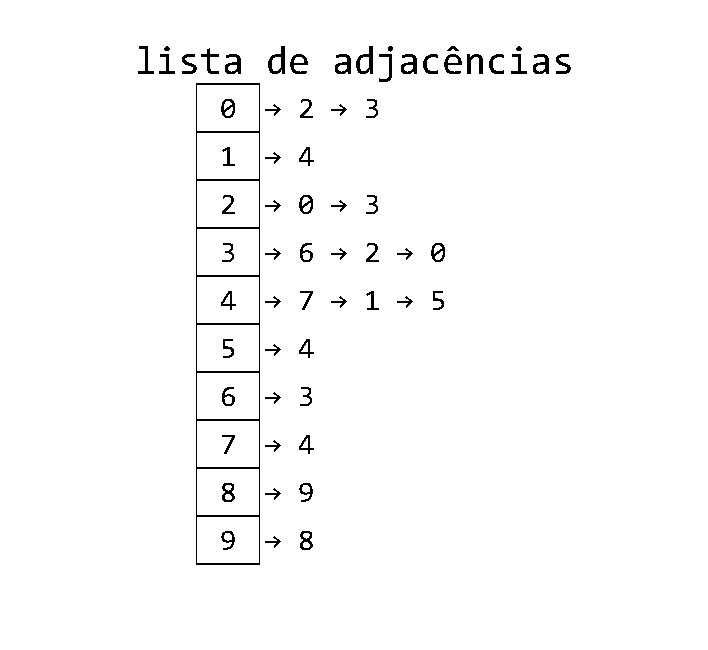
\includegraphics[width=.32\textwidth]{figB.pdf}
	}
	\subcaptionbox{}[.32\textwidth]
	{
		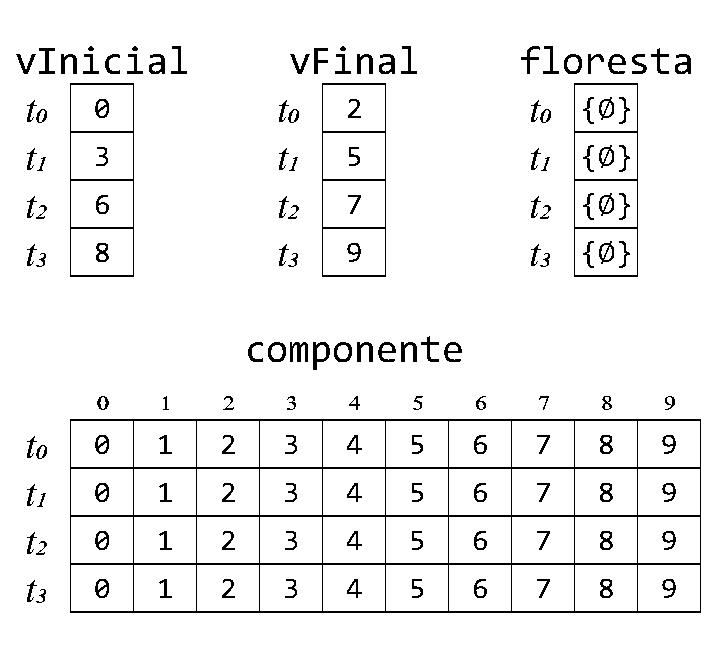
\includegraphics[width=.32\textwidth]{figC.pdf}
	}
	\subcaptionbox{}[.32\textwidth]
	{
		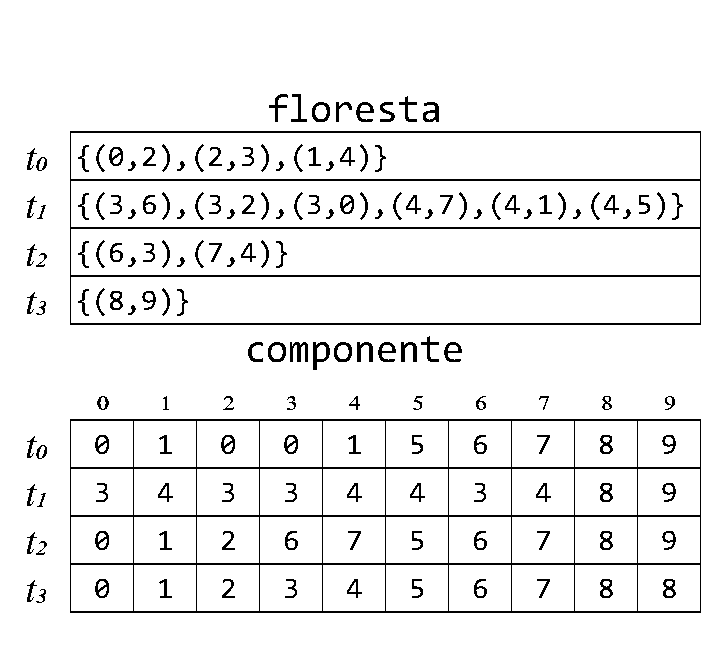
\includegraphics[width=.32\textwidth]{figD.pdf}
	}
	\subcaptionbox{}[.32\textwidth]
	{
		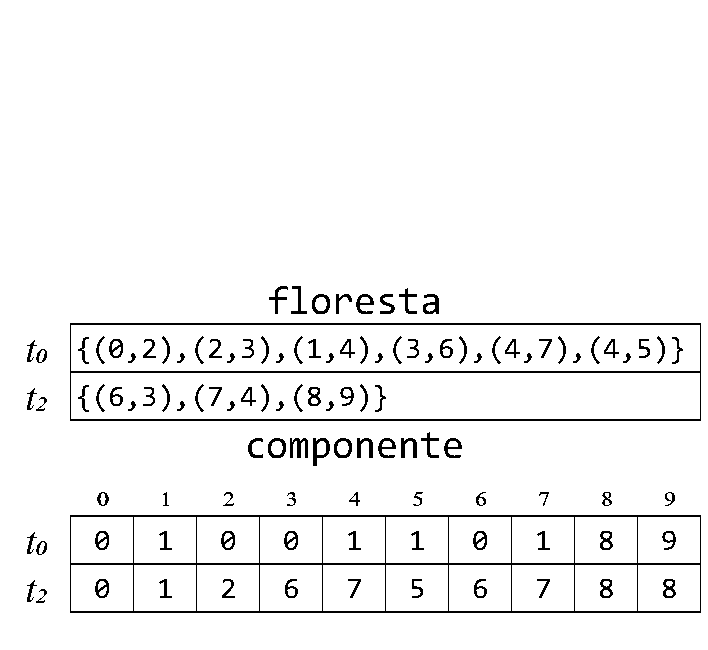
\includegraphics[width=.32\textwidth]{figE.pdf}
	}
	\subcaptionbox{}[.32\textwidth]
	{
		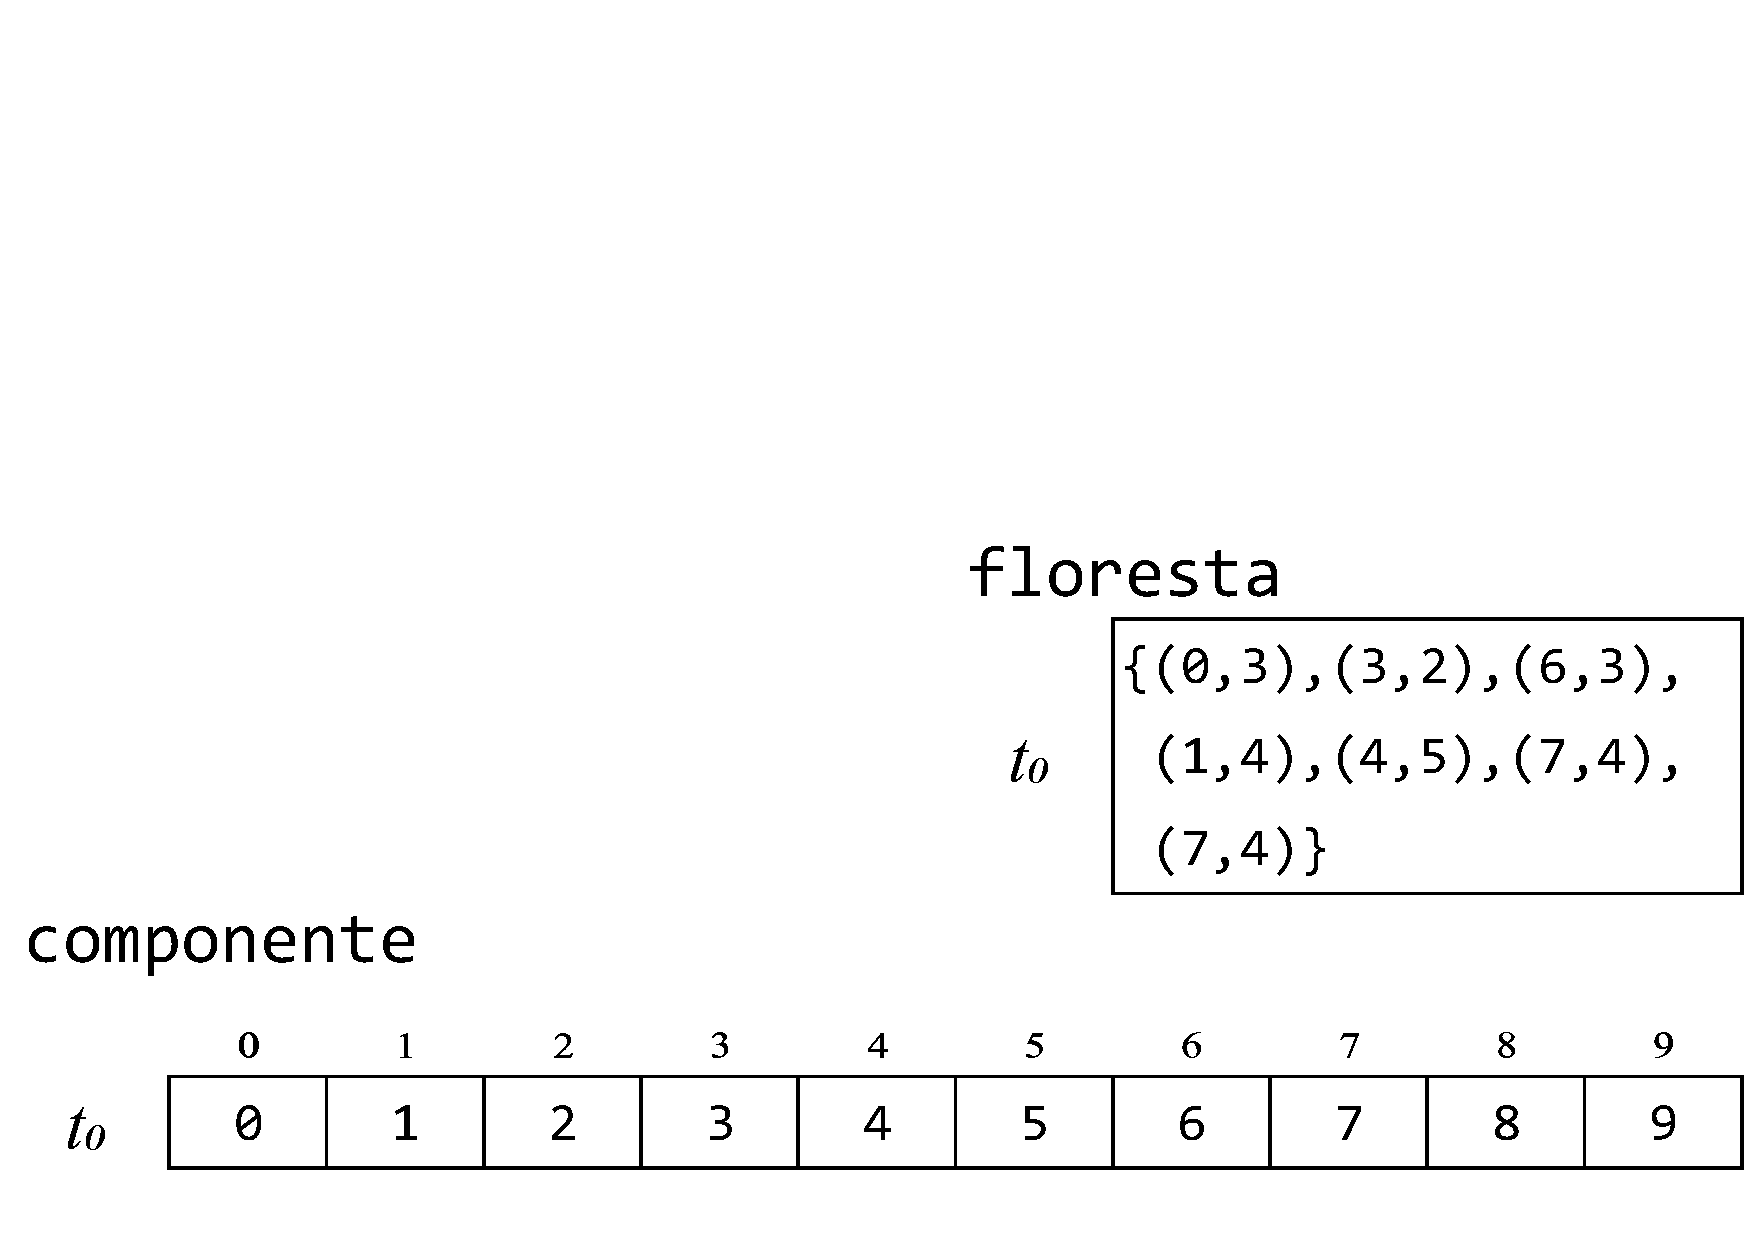
\includegraphics[width=.32\textwidth]{figF.pdf}
	}
	\caption{Passos da execução da implementação paralela, com quatro threads: (a) Grafo de entrada G; (b) Lista de adjacências de G; (c) Estruturas de dados antes da busca em profundidade em paralelo; (d) Estruturas de dados após a busca em profundidade em paralelo; (e) Estruturas de dados após o primeiro passo de uniões em paralelo; (f) Estruturas de dados após o segundo passo de uniões (resultado final da implementação).}
		\label{fig:1}
\end{figure}

Os Algoritmos~\ref{alg_par1} e~\ref{alg_par2} apresentam a implementação paralela desenvolvida, usando a busca em profundidade e as operações \emph{Union-Find}.

\begin{algorithm}[H]
    \DontPrintSemicolon
    \SetArgSty{textnormal}
    \newcommand\mycommfont[1]{\small\ttfamily{#1}}
	\SetCommentSty{mycommfont}
    %\SetAlCapNameFnt{\small} %tamanho nome do algoritmo
    \caption{Implementação do algoritmo paralelo para componentes conexos}
    \label{alg_par1}
    \SetKwProg{ComponentesConexosPar}{ComponentesConexosParalelo}{}{}
    \SetKwFor{ForPar}{para}{fa\c{c}a em paralelo}{fim para cada}
    \ComponentesConexosPar{{\normalfont(grafo G = (V, E))}}
    {
    	\tcp{Divida os vértices pelas threads}
        nTh $\gets$ número de threads\;
        nVerticesExtra $\gets |\text{V}|$ -- ($\lfloor \frac{|\text{V}|}{\text{nTh}} \rfloor$ $\times$ nTh)\;
        \ForPar{t $\gets$ 0 \Ate nTh -- 1}
        {
            \eSe{t $<$ nVerticesExtra}
            {
                vInicial[t] $\gets$ t $\times$ $\lceil\frac{|\text{V}|}{\text{nTh}}\rceil$\;
                vFinal[t] $\gets$ vInicial[t] + $\lceil\frac{|\text{V}|}{\text{nTh}}\rceil$ -- 1\;
            }
           {
                vInicial[t] $\gets$ t $\times$ $\lfloor\frac{|\text{V}|}{\text{nTh}}\rfloor$ + nVerticesExtra\;
                vFinal[t] $\gets$ vIncial[t] + $\lfloor\frac{|\text{V}|}{\text{nTh}}\rfloor$ -- 1\;
            }
        }
        \tcp{Execute DFS em paralelo, gerando nTh florestas}
        \ParaCada{vértice v $\in$ V}
        {
            visitado[v] $\gets$ FALSO\;
        }
        \ForPar{t $\gets$ 0 \Ate nTh -- 1}
        {
            \ParaCada{vértice v $\in$ V}
            {
                componente[t][v] $\gets$ v\;
            }
            floresta[t] $\gets$ \{$\emptyset$\}\;
            \Para{v $\gets$ vInicial[t] \Ate vFinal[t]}
            {
                \Se{visitado[v] = FALSO}
                {
                    raiz $\gets$ v\;
                    \textbf{DFS}(t, v, raiz)\;
                }
            }
        }
        \tcp{Una pares de florestas em paralelo}
        nPares $\gets \frac{\text{nTh}}{\text{2}}$\;
        \Para{i $\gets$ 0 \Ate $\log_2\!\text{(nTh)}$ -- 1}
        {
            \ForPar{t $\gets$ 0 \Ate nPares -- 1}
            {
                thEsquerda $\gets$ t $\times$ $\text{2}^{\text{i+1}}$\;
                thDireita $\gets$ thEsquerda + $\text{2}^\text{i}$\;
                
                \ParaCada{aresta (v, u) $\in$ floresta[thDireita]}
                {
                    \textbf{Union}(thEsquerda, v, u)\;
                }
            }
            nPares $\gets \frac{\text{nPares}}{\text{2}}$\;
        }
    }
    \SetKwProg{DFS}{DFS}{}{}
    \DFS{{\normalfont(thread t, vértice v, vértice raiz)}}
    {
        componente[t][v] $\gets$ raiz\;
        visitado[v] $\gets$ VERDADEIRO\;
        
        \ParaCada{vértice u $\in$ Adj[v]}
        {
            floresta[t] $\gets$ floresta[t] $\cup$ \{(v, u)\}\;
            componente[t][u] $\gets$ raiz\;
            
            \Se{vInicial[t] $\le$ u \textbf{\upshape e} u $\le$ vFinal[t]}
            {
                \Se{visitado[u] = FALSO}
                {
                    \textbf{DFS}(t, u, raiz)\;
                }
            }
        }
    }
\end{algorithm}
    
\begin{algorithm}[!htb]
    \DontPrintSemicolon
    \SetArgSty{textnormal}
    \caption{Operações Union e Find}
    \label{alg_par2}
    \SetKw{Return}{retorna}
    \SetKwProg{UNION}{Union}{}{}
    \UNION{{\normalfont(thread t, vértice v, vértice u)}}
    {
        vComponente $\gets$ \textbf{Find}(t, v)\;
        uComponente $\gets$ \textbf{Find}(t, u)\;
        \Se{vComponente $\neq$ uComponente}
        {
            min $\gets$ \textbf{Mínimo}(vComponente, uComponente)\;
		    max $\gets$ \textbf{Máximo}(vComponente, uComponente)\;
            \ParaCada{vértice i $\in$ V}
            {
                \Se{componente[t][i] = max}
                {
                    componente[t][i] $\gets$ min\;
                }
            }
            floresta[t] $\gets$ floresta[t] $\cup$ \{(v, u)\}\;
        }
    }
    \SetKwProg{FIND}{Find}{}{}
    \FIND{{\normalfont(thread t, vértice v)}}
    {
        \Return componente[t][v]\;
    }
\end{algorithm}

%--------------------------------------------------------------------------------
\section{Resultados e Análise}
\label{resultados}

Para mensurar o desempenho dos algoritmos sequencial e paralelo implementados, foram utilizados como entrada grafos gerados aleatoriamente. A fim de observar o comportamento dos algoritmos com diferentes tipos de grafos, foram utilizados grafos com diferentes quantidade de vértices e densidade. Define-se nesse trabalho a densidade de um grafo como a proporção da sua quantidade de arestas em relação à quantidade de arestas do grafo completo com o mesmo número de vértices. Foram gerados grafos com 5.000, 10.000, 15.000 e 25.000 vértices. Apesar das quantidades de vértices serem aparentemente pequenas, os algoritmos analisam todas as arestas do grafo e não somente os vértices. Por exemplo, para um grafo completo de 25.000 vértices, há mais de 312 milhões de arestas. As densidades escolhidas foram 10\%, 25\%, 50\%, 75\% e 100\%. Um grafo de $n$ vértices de densidade 100\% é simplesmente o grafo completo $K_n$. Um grafo de $n$ vértices de densidade 10\% possui um número de arestas igual a 10\% das arestas do grafo $K_n$. Por exemplo, um grafo de 5.000 vértices e densidade de 25\%, possui 3.124.375 arestas.

O computador usado na avaliação de desempenho é um Dell Precision, com processador Intel Xeon E5-1620 v3 3,5GHz, com 4 núcleos e 8 threads, e 32 GB de RAM. Foram utilizados o compilador GCC versão 7.4 (com a opção de otimização -O3) e o sistema operacional Ubuntu 16.04 x86\_64. Os resultados apresentados foram obtidos a partir de cinco execuções de cada algoritmo, para cada quantidade de vértices e densidade do grafo de entrada.

As Figuras~\ref{fig:2}(a) e \ref{fig:2}(b) comparam os tempos de execução dos algoritmos sequencial e paralelo, esse último usando 16 \emph{threads}, para as diferentes entradas. Na Figura~\ref{fig:2}(a), a densidade do grafo de entrada é fixada em 100\% e na Figura~\ref{fig:2}(b) a quantidade de vértices do grafo de entrada é fixado em 25.000 vértices. É possível notar que o tempo de execução do algoritmo sequencial aumenta exponencialmente quando se varia a quantidade de vértices, enquanto que, no algoritmo paralelo, apesar de não ser linear, o aumento do tempo de execução é bem menor. Também se observa que a densidade do grafo de entrada impacta muito mais o tempo de execução do algoritmo sequencial do que o tempo do algoritmo paralelo.

\begin{figure}[!htb]
    \centering
    \begin{minipage}{.48\textwidth}
        \centering
        \resizebox{\textwidth}{!}
        {
			\begin{tikzpicture}
			\begin{axis}[
				%title={Execução alg par 25k com várias threads},
				legend pos=north west,
				xlabel={quantidade de vértices},
				%legend style={at={(0.5,-0.20)},anchor=north,legend columns=-1},
				%symbolic x coords={a,b,c,d},
				ylabel={tempo de execução (s)},
				xtick=data,
				symbolic x coords={5K, 10K, 15K, 25K}]
				\addplot coordinates {
					(5K,2.8425)(10K,12.9809)(15K,35.0820)(25K,105.7478)};
				\addplot coordinates {
					(5K,0.9850)(10K,4.2318)(15K,10.5094)(25K,30.9745)};
			\legend{Sequencial, Paralelo}
			\end{axis}
			\end{tikzpicture}
		}
        \subcaption{}
    \end{minipage}\hfill%
    \begin{minipage}{.48\textwidth}
        \centering
        \resizebox{\textwidth}{!}
        {
			\begin{tikzpicture}
			\begin{axis}[
				%title={Execução alg par 25k com várias threads},
				legend pos=north west,
				xlabel={densidade do grafo},
				%legend style={at={(0.5,-0.20)},anchor=north,legend columns=-1},
				%symbolic x coords={a,b,c,d},
				ylabel={tempo de execução (s)},
				xtick=data,
				symbolic x coords={5\%, 25\%, 50\%, 75\%, 100\%}]
				\addplot coordinates {
					(5\%,3.7357)(25\%,22.9317)(50\%,50.8209)(75\%,77.6357)(100\%,105.7478)};
				\addplot coordinates {
					(5\%,1.3433)(25\%,8.1235)(50\%,16.6858)(75\%,24.3761)(100\%,30.9745)};
			\legend{Sequencial, Paralelo}
			\end{axis}
			\end{tikzpicture}
		}
        \subcaption{}
    \end{minipage}
    \caption{Tempo de execução das soluções sequencial e paralela (com 16 \emph{threads}): (a) variando quantidade de vértices e densidade fixa em 100\%; (b) variando densidade e quantidade de vértices fixa em 25.000}
    \label{fig:2}
\end{figure}

As Figuras~\ref{fig:3}(a) e~\ref{fig:3}(b) mostram os \emph{speedups} alcançados pelo algoritmo paralelo (usando 16 \emph{threads}) em relação ao algoritmo sequencial. Nas duas figuras, os resultados para todos os grafos de entrada são mostrados, variando apenas o eixo de exibição. É interessante notar que há uma variação de desempenho para os grafos de 5.000 e 10.000 vértices com densidade de 25\%, já  que ele não segue o “padrão” visto para os outros grafos de entrada. Inicialmente, pensou-se que isso se devia a um caso isolado, mas após várias execuções, esse desempenho se repetiu. Também se observa que o algoritmo paralelo, com o maior e mais denso grafo de entrada, foi 3,4 vezes mais rápido que o algoritmo sequencial.

\begin{figure}[!htp]
    \centering
    \begin{minipage}{.48\textwidth}
        \centering
        \resizebox{\textwidth}{!}
        {
			\begin{tikzpicture}
			\begin{axis}[
				%title={Execução alg par 25k com várias threads},
				legend style={at={(0.5,1.15)},anchor=north,legend columns=-1},
				xlabel={quantidade de vértices},
				%legend style={at={(0.5,-0.20)},anchor=north,legend columns=-1},
				%symbolic x coords={a,b,c,d},
				ylabel={\emph{speedup}},
				xtick=data,
				symbolic x coords={5K, 10K, 15K, 25K}]
				\addplot coordinates {
					(5K,2.0066)(10K,2.5546)(15K,2.5800)(25K,2.7810)};
				\addplot coordinates {
					(5K,2.7384)(10K,2.7336)(15K,2.6243)(25K,2.8229)};
				\addplot coordinates {
					(5K,2.6475)(10K,2.7354)(15K,2.7931)(25K,3.0458)};
				\addplot coordinates {
					(5K,2.7349)(10K,2.8928)(15K,3.0592)(25K,3.1849)};
				\addplot+[green, mark options={fill=green}] coordinates {
					(5K,2.8858)(10K,3.0675)(15K,3.3382)(25K,3.4140)};
			\legend{5\%, 25\%, 50\%, 75\%, 100\%}
			\end{axis}
			\end{tikzpicture}
		}
        \subcaption{}
    \end{minipage}\hfill%
    \begin{minipage}{.48\textwidth}
        \centering
        \resizebox{\textwidth}{!}
        {
			\begin{tikzpicture}
			\begin{axis}[
				legend pos=north west,
				%legend style={at={(0.5,1.15)},anchor=north,legend columns=-1},
				%xlabel={densidade do grafo},
				%legend style={at={(0.5,-0.20)},anchor=north,legend columns=-1},
				%symbolic x coords={a,b,c,d},
				ylabel={\emph{speedup}},
				xlabel={densidade do grafo},
				xtick=data,
				symbolic x coords={5\%, 25\%, 50\%, 75\%, 100\%}]
				\addplot coordinates {
					(5\%,2.0066)(25\%,2.7384)(50\%,2.6475)(75\%,2.7349)(100\%,2.8858)};
				\addplot coordinates {
					(5\%,2.5546)(25\%,2.7336)(50\%,2.7354)(75\%,2.8928)(100\%,3.0675)};
				\addplot coordinates {
					(5\%,2.5800)(25\%,2.6243)(50\%,2.7931)(75\%,3.0592)(100\%,3.3382)};
				\addplot coordinates {
					(5\%,2.7810)(25\%,2.8229)(50\%,3.0458)(75\%,3.1849)(100\%,3.4140)};
			\legend{5K, 10K, 15K, 25K}
			\end{axis}
			\end{tikzpicture}
		}
        \subcaption{}
    \end{minipage}
    \caption{\emph{Speedup} da solução paralela (com 16 \emph{threads}) em relação à sequencial: (a) e (b) variando quantidade de vértices e densidade}
    \label{fig:3}
\end{figure}

Por padrão, o OpenMP utiliza a quantidade de \emph{threads} disponíveis do processador. A fim de experimentação, quantidades diferentes de \emph{threads} foram escolhidas para analisar o comportamento do algoritmo paralelo. Como é visto nas Figuras~\ref{fig:4}(a) e~\ref{fig:4}(b), o melhor resultado de tempo de execução foi obtido ao utilizar 16 \emph{threads}. Apesar de não haver diferença expressiva entre o uso de 8 ou 16 \emph{threads}, a execução com 16 \emph{threads} obteve o melhor desempenho.

\begin{figure}[!htp]
    \centering
    \begin{minipage}{.48\textwidth}
        \centering
        \resizebox{\textwidth}{!}
        {
			\begin{tikzpicture}
			\begin{axis}[
				legend pos=north west,
				xlabel={quantidade de vértices},
				%legend style={at={(0.5,-0.20)},anchor=north,legend columns=-1},
				%symbolic x coords={a,b,c,d},
				ylabel={tempo de execução (s)},
				xtick=data,
				symbolic x coords={5K, 10K, 15K, 25K}]
				\addplot coordinates {
					(5K,2.0038)(10K,8.4621)(15K,21.8479)(25K,64.3706)};
				\addplot coordinates {
					(5K,1.2820)(10K,5.8591)(15K,14.8007)(25K,41.4975)};
				\addplot+[green, mark options={fill=green}] coordinates {
					(5K,1.0018)(10K,4.3181)(15K,10.5758)(25K,31.0767)};
				\addplot coordinates {
					(5K,0.9850)(10K,4.2318)(15K,10.5094)(25K,30.9745)};
			\legend{2 $th$,4 $th$,8 $th$, 16 $th$}
			\end{axis}
			\end{tikzpicture}
		}
        \subcaption{}
    \end{minipage}\hfill%
    \begin{minipage}{.48\textwidth}
        \centering
        \resizebox{\textwidth}{!}
        {
			\begin{tikzpicture}
			\begin{axis}[
				legend pos=north west,
				xlabel={densidade do grafo},
				%legend style={at={(0.5,-0.20)},anchor=north,legend columns=-1},
				%symbolic x coords={a,b,c,d},
				ylabel={tempo de execução (s)},
				%xtick=data,
				symbolic x coords={5\%, 25\%, 50\%, 75\%, 100\%}]
				\addplot coordinates {
					(5\%,2.4396)(25\%,15.6663)(50\%,33.4889)(75\%,51.2299)(100\%,64.3706)
				};
				\addplot coordinates {
					(5\%,1.6939)(25\%,11.2393)(50\%,22.2700)(75\%,35.0567)(100\%,41.4975)
				};
				\addplot+[green, mark options={fill=green}] coordinates {
					(5\%,1.3561)(25\%,8.1547)(50\%,16.7268)(75\%,24.5019)(100\%,31.0767)
				};
				\addplot coordinates {
					(5\%,1.3433)(25\%,8.1235)(50\%,16.6858)(75\%,24.3761)(100\%,30.9745)
				};
			\legend{2 $th$,4 $th$,8 $th$, 16 $th$}
			\end{axis}
			\end{tikzpicture}
		}
        \subcaption{}
    \end{minipage}
    \caption{Tempo de execução da solução paralela: (a) variando quantidade de vértices e número de \emph{threads}, densidade fixa em 100\%; (a) variando densidade e número de \emph{threads}, quantidade de vértices fixa em 25.000}
    \label{fig:4}
\end{figure}

%--------------------------------------------------------------------------------
\section{Conclusão}
\label{conclusao}

A descrição do algoritmo paralelo em~\cite{Grama:2003} é muito alto nível, em especial na união das florestas. Assim, projetar e implementar esse algoritmo mostrou-se ser desafiador. As estruturas de dados utilizadas e a maneira como foi implementada a união das florestas, foram concebidas no desenvolvimento deste trabalho. Em contrapartida, utilizar o modelo de programação paralela OpenMP facilitou muito a implementação do paralelismo no algoritmo. Não foram realizados experimentos com grafos com mais de 25.000 vértices, devido a limitações de memória do computador utilizado.

O algoritmo paralelo teve um ganho de desempenho de até 3,4 vezes em relação ao sequencial. Ao analisar que o processador usado possui apenas 4 núcleos, esse ganho é muito satisfatório. Mesmo no pior cenário, o algoritmo paralelo alcançou pelo menos 2 vezes o desempenho do algoritmo sequencial. Apesar das complexidades maiores que o algoritmo paralelo traz em relação ao sequencial (que é bastante simples e muito bem conhecido na literatura), o desempenho obtido compensa a dificuldade e põe o algoritmo paralelo como uma boa escolha para resolver o problema dos componentes conexos.

Como trabalhos futuros, é possível melhorar ainda mais a implementação do algoritmo paralelo. As operações \emph{Union-Find} utilizadas na implementação são as mais simples da literatura. Em~\cite{Sedgewick:2011} é apresentada uma versão mais eficiente dessas operações, com pesos e compressão de caminhos, porém, de maior complexidade de implementação. Outra questão no algoritmo paralelo aqui implementado é em relação à união de florestas. A cada passo realizado de uniões par a par, metade das \emph{threads} deixam de ser usadas no próximo passo. Projetar uma maneira de utilizar novamente essas \emph{threads} possui o potencial de trazer um ganho de desempenho ainda maior para o algoritmo paralelo.

%--------------------------------------------------------------------------------
\bibliographystyle{sbc}
\bibliography{sbc-template}

%--------------------------------------------------------------------------------
\end{document}
%--------------------------------------------------------------------------------
